\documentclass[11pt,a4paper]{article}
\usepackage{fullpage}
\usepackage[T1]{fontenc} 
\usepackage[utf8]{inputenc}
\usepackage{amsmath}
\usepackage{amssymb}
\usepackage{float}
\usepackage{tabularx}
\usepackage{multirow}
\usepackage{graphicx}
\usepackage{geometry}
\usepackage[table,dvipsnames]{xcolor}
\usepackage[hidelinks]{hyperref}
\usepackage[polish]{babel}
\usepackage{menukeys}
\usepackage{subcaption}

\setlength{\parindent}{0cm}
\setlength{\parskip}{2mm}
\newcolumntype{Y}{>{\centering\arraybackslash}X}
\DeclareMathOperator{\sgn}{sgn}

\begin{document}

\title{Rozpoznawanie człowieka metodami biometrii \\
\Large{
    Projekt 2. --- Rozpoznawanie na~podstawie głosu \\
    Raport
}}
\author{Bartłomiej Dach}
\maketitle

Poniższy dokument stanowi sprawozdanie z~implementacji aplikacji dokonującej rozpoznawania człowieka na~podstawie zarejestrowanych próbek głosu.
W~dokumencie opisano zastosowaną metodę opartą na~współczynnikach mel-cepstralnych oraz~zawarto wyniki działania dla~próbek zarejestrowanych przez~studentów uczęszczających na~zajęcia.

\section{Wstęp}

Ludzki głos jest cechą biometryczną z~pogranicza cech biologicznych i~behawioralnych.
Podczas gdy barwa głosu jest determinowana przez~wrodzone czynniki anatomiczne, ton głosu i~akcent stosowany podczas~wymawiania określonych fraz stanowi cechę nabytą podczas nauki mowy.

Rozpoznawanie człowieka na~podstawie mowy to~prężnie rozwijające~się zagadnienie.
Ze~względu na~rosnącą popularność urządzeń interpretujących frazy wymawiane przez~użytkowników takich, jak~Google Home czy~Amazon Echo, identyfikacja na~podstawie głosu stanowi ważny kierunek rozwoju.

W~ramach projektu zaimplementowano prostą metodę klasyfikacji próbek na~podstawie danego wcześniej zbioru treningowego, używającą współczynników mel-cepstralnych.
Szczegółowy opis metody znajduje~się w~sekcji~\ref{sec:method}.

\section{Opis aplikacji}

\subsection{Zastosowane biblioteki}

\begin{table}
    \begin{tabularx}{\textwidth}{|r|l|X|l|c|}
        \hline
        Nr & Nazwa & Opis & Licencja & \\
        \hline
        \hline
        1 & \texttt{matplotlib} 3.0.3 & Tworzenie wykresów i~wizualizacji & PSF & \cite{hunter2007} \\
        \hline
        2 & \texttt{numpy} 1.16.2 & Wielowymiarowe tablicowe struktury danych & BSD & \cite{oliphant2006} \\
        \hline
        3 & \texttt{pandas} 0.24.2 & Struktury do~manipulacji i~analizy danych & BSD & \cite{mckinney2010} \\
        \hline
        4 & \texttt{seaborn} 0.9.0 & Rozszerzone wizualizacje danych & BSD & \cite{waskom2018} \\
        \hline
        5 & \texttt{scipy} 1.2.1 & Algorytmy pomocnicze (transformata Fouriera, manipulacja dźwiękiem) & BSD & \cite{jones2001} \\
        \hline
    \end{tabularx}
    \caption{Lista bibliotek użytych w~projekcie}
    \label{tbl:libraries}
\end{table}

\subsection{Instrukcja obsługi}

\section{Opis metody}
\label{sec:method}

\subsection{Wyznaczanie współczynników mel-cepstralnych}

\subsection{Klasyfikacja nowych próbek}

\section{Wyniki eksperymentalne}

\begin{figure}
    \centering
    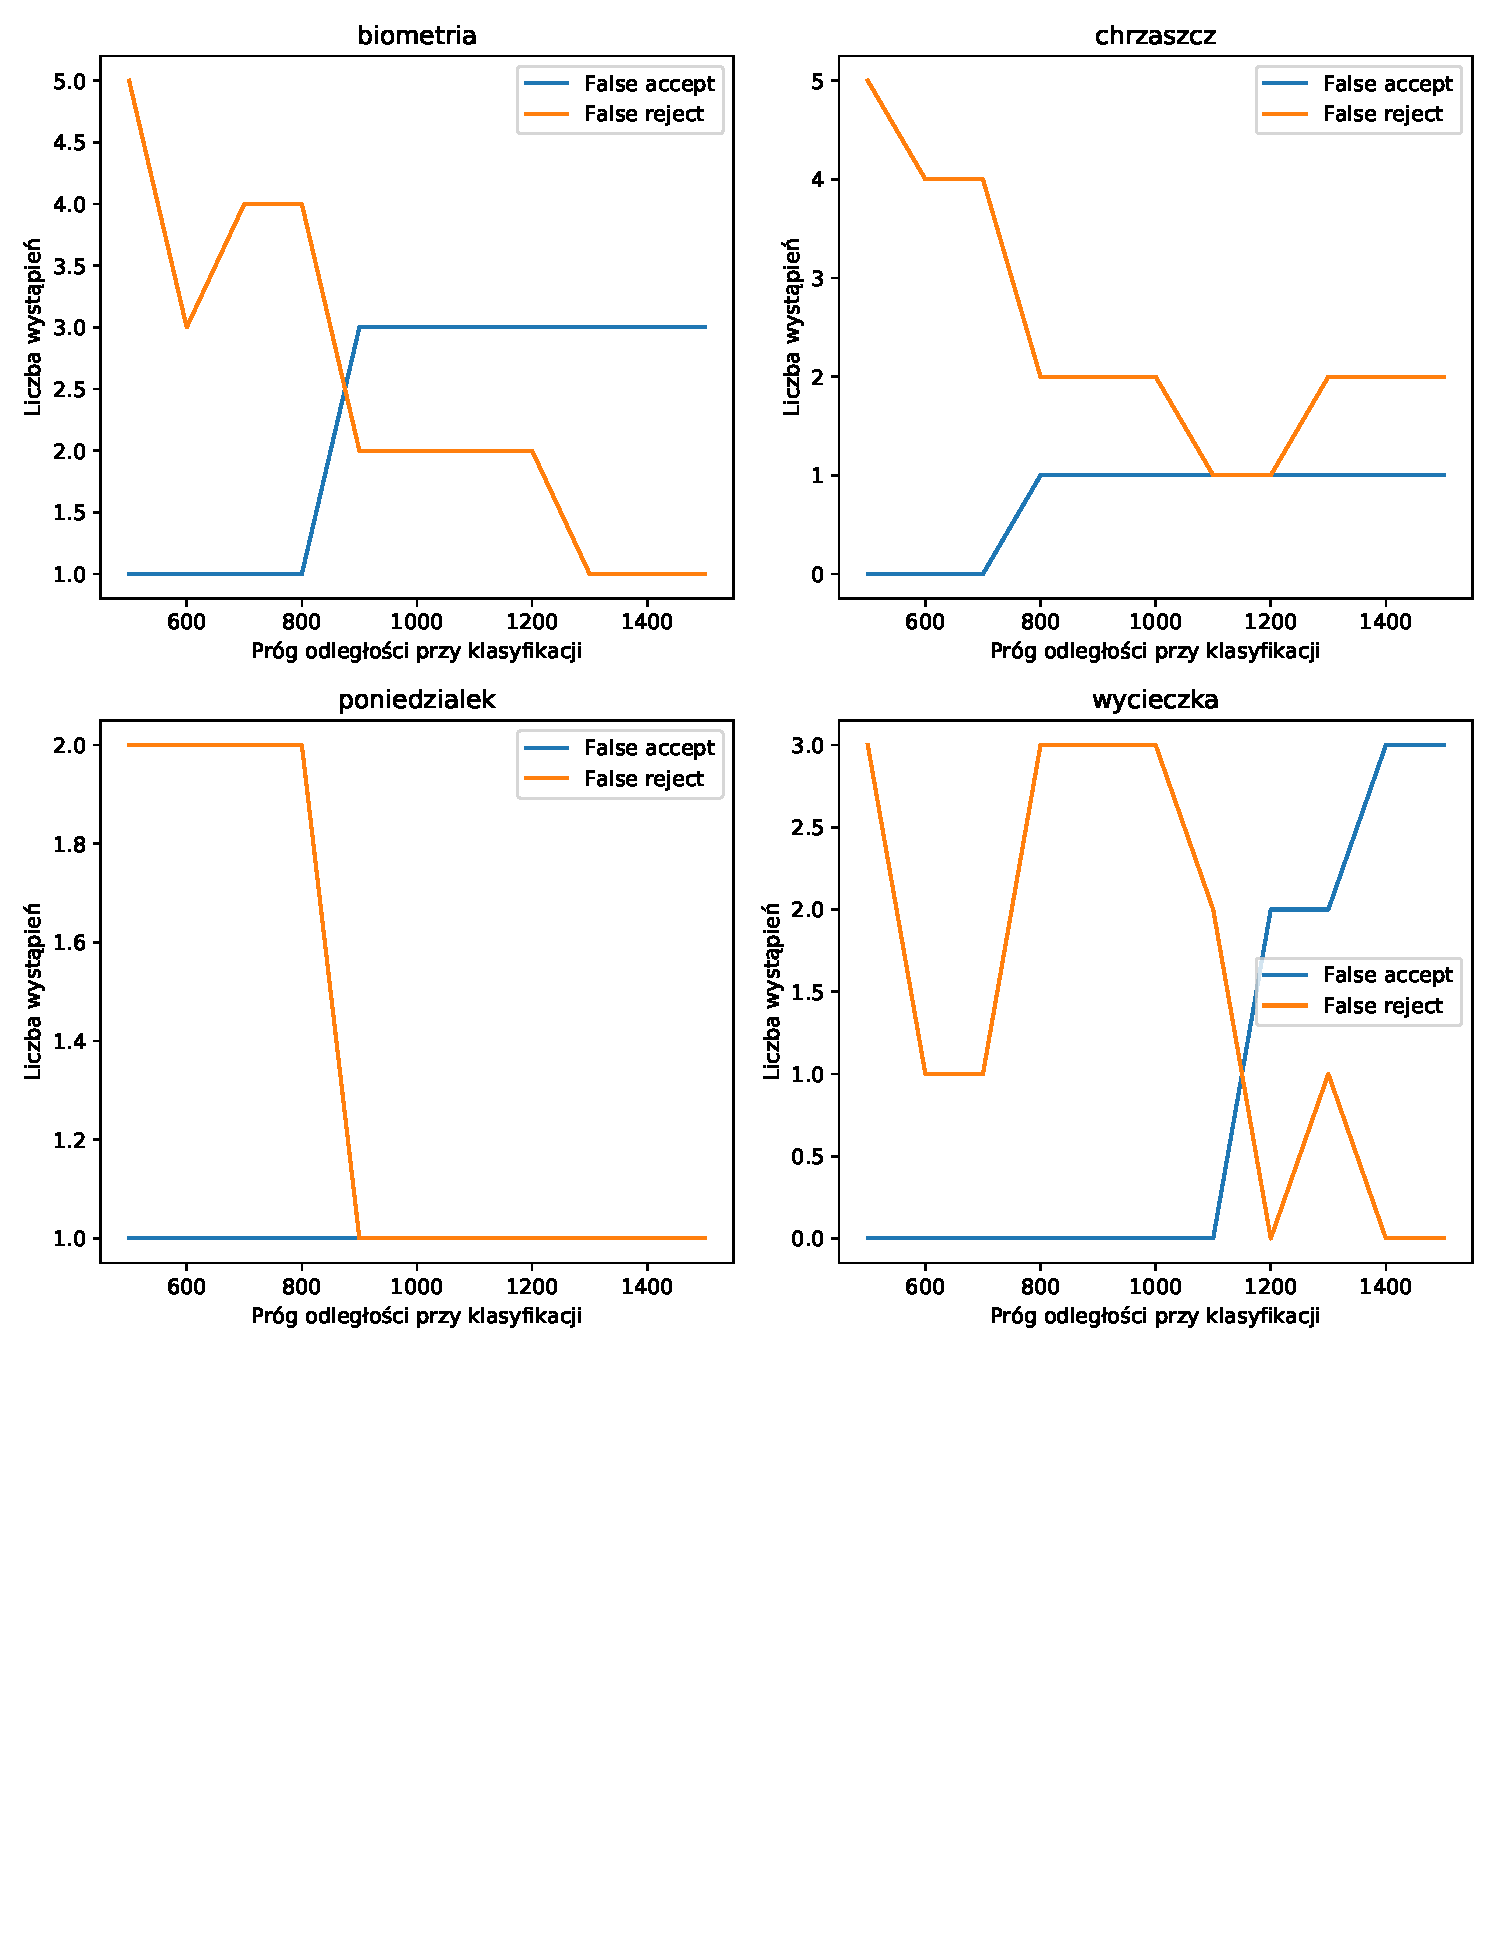
\includegraphics[width=\textwidth]{res/plots/acceptance_rates.pdf}
    \caption{Liczba fałszywych pozytywów (ang.~\emph{false accept}) i~fałszywych odrzuceń (ang.~\emph{false reject}) próbek głosów z~testowanego zbioru w~zależności od~przyjętego progu odległości między~próbkami podczas klasyfikacji.
    Oddzielono wyniki dla~każdej z~czterech rejestrowanych fraz.}
    \label{fig:acceptance-rates}
\end{figure}

\begin{figure}
    \centering
    \begin{subfigure}[t]{0.45\textwidth}
        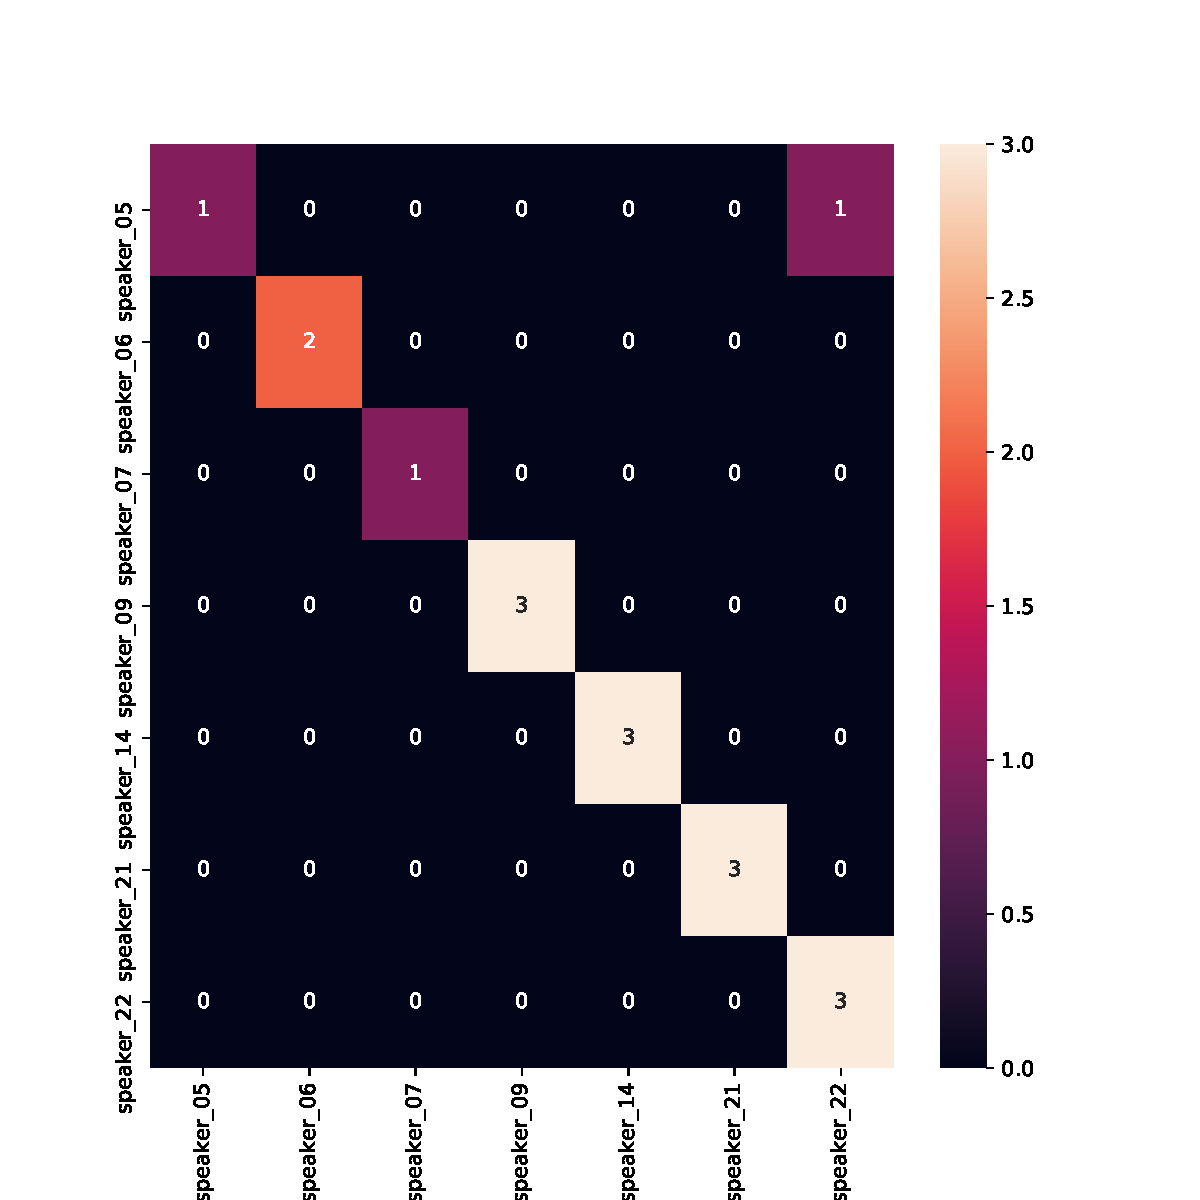
\includegraphics[width=\textwidth]{res/plots/confusion_matrix_biometria.pdf}
        \caption{Macierz pomyłek dla~słowa \emph{biometria} przy~progu~$t = 800$.}
    \end{subfigure}
    \qquad
    \begin{subfigure}[t]{0.45\textwidth}
        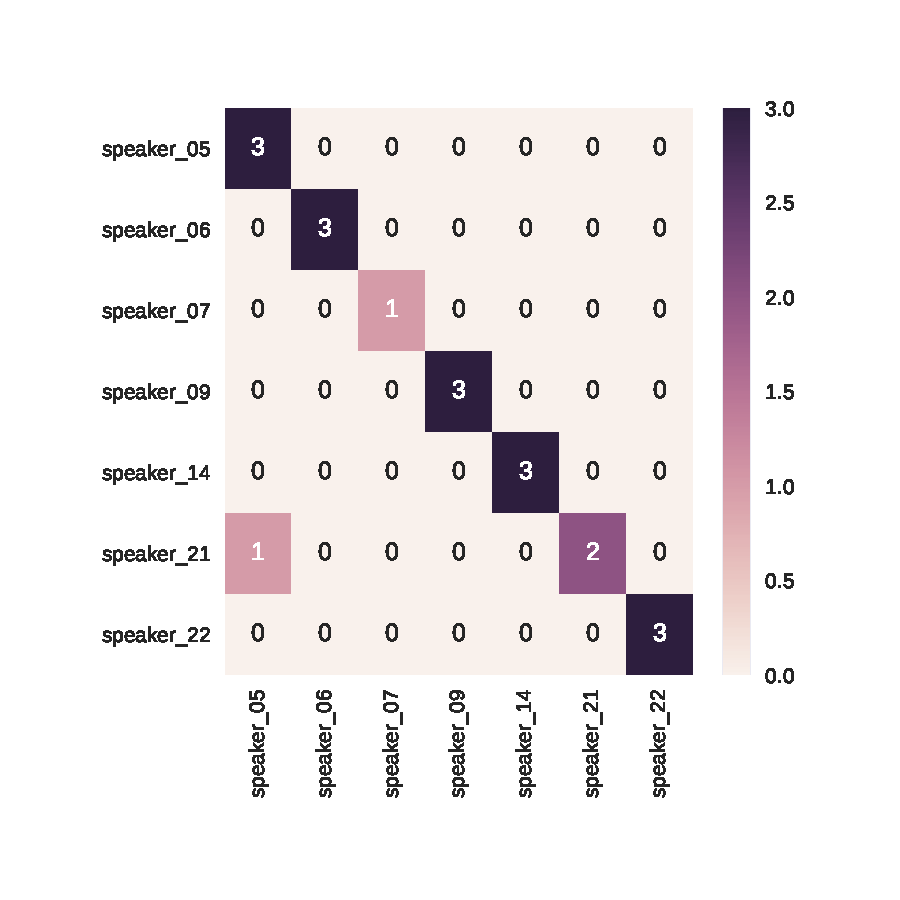
\includegraphics[width=\textwidth]{res/plots/confusion_matrix_chrzaszcz.pdf}
        \caption{Macierz pomyłek dla~słowa \emph{chrząszcz} przy~progu~$t = 800$.}
    \end{subfigure}
    \\
    \begin{subfigure}[t]{0.45\textwidth}
        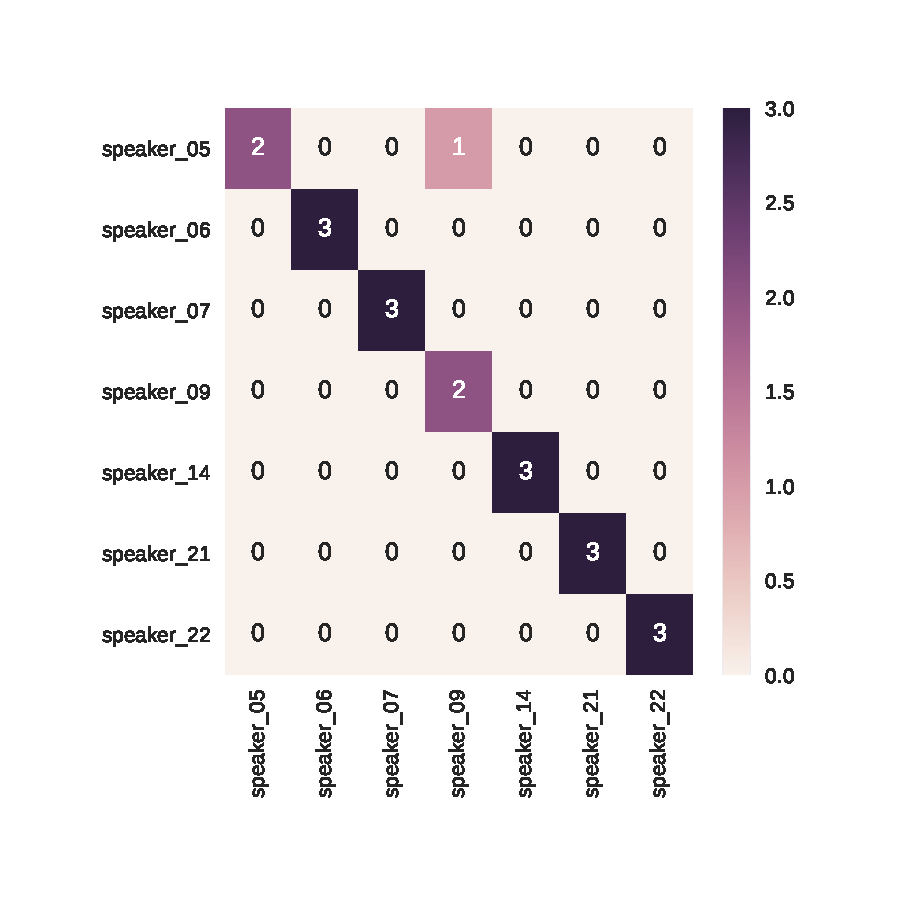
\includegraphics[width=\textwidth]{res/plots/confusion_matrix_poniedzialek.pdf}
        \caption{Macierz pomyłek dla~słowa \emph{poniedziałek} przy~progu~$t = 900$.}
    \end{subfigure}
    \qquad
    \begin{subfigure}[t]{0.45\textwidth}
        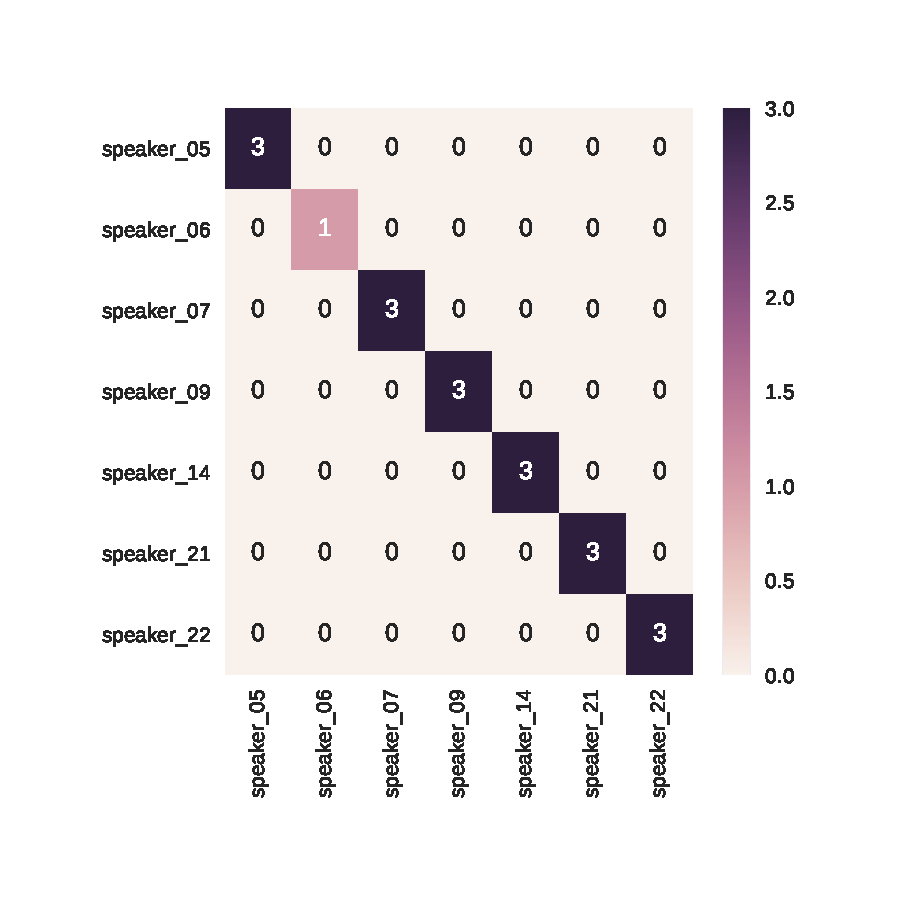
\includegraphics[width=\textwidth]{res/plots/confusion_matrix_wycieczka.pdf}
        \caption{Macierz pomyłek dla~zdania \emph{Jutro pojadę na~wycieczkę, albo~zostanę w~domu} przy~progu~$t = 1100$.}
    \end{subfigure}
    \caption{Macierze pomyłek dla~wartości progu minimalizujących liczbę fałszywych pozytywów i~negatywów dla~poszczególnych zarejestrowanych fraz.}
\end{figure}

\section{Podsumowanie}

\begin{thebibliography}{9}

    \bibitem{hunter2007}
        Hunter, J.D.,
        ,,Matplotlib: A~2D~graphics environment'',
        \emph{Computing In~Science \& Engineering},
        tom~9,
        nr~3,
        s.~90--95,
        2007.

    \bibitem{jones2001}
        Jones, E., Oliphant T.E., Peterson P. i~inni,
        ,,SciPy: Open source scientific tools for~Python''.
        [Online]
        \\
        Dostępne: \url{https://www.scipy.org/}.
        [Dostęp 7 kwietnia 2019]

    \bibitem{mckinney2010}
        McKinney, W.,
        ,,Data Structures for~Statistical Computing in~Python'',
        \emph{Proceedings of~the~9\textsuperscript{th} Python in~Science Conference},
        s.~51--56,
        2010.

    \bibitem{oliphant2006}
        Oliphant, T.E.,
        \emph{A Guide to NumPy},
        Trelgol~Publishing,
        Stany Zjednoczone,
        2006.

    \bibitem{waskom2018}
        Waskom, M. i~inni,
        ,,\texttt{seaborn}: statistical data visualization''.
        [Online]
        \\
        Dostępne: \url{https://seaborn.pydata.org/}.
        [Dostęp 7 kwietnia 2019]

    %\bibitem{slot2008}
        %Ślot K.,
        %\emph{Wybrane zagadnienia biometrii},
        %Wydawnictwa Komunikacji i~Łączności,
        %Warszawa 2008.

\end{thebibliography}

\end{document}
